\section{Introduction: Generalized Parton Distributions and DVCS}
Generalized Parton Distributions (GPDs) are nowadays the object of an intense 
effort of research, in the perspective of understanding nucleon structure.
The GPDs describe the correlations between the longitudinal momentum and transverse spatial position of the partons inside the nucleon, they give access to
the contribution of the orbital momentum of the quarks to the nucleon, and they are sensitive to the correlated $q-\bar{q}$ components.
The original articles and general reviews on GPDs and details of the formalism can be found in Refs.~\cite{muller}-\cite{revrady}.%~\cite{muller,ji,rady,collins,goeke,revdiehl,revrady}.

The nucleon GPDs are accessed in the measurement of the exclusive leptoproduction of a photon (DVCS, which stands for deeply virtual Compton scattering) or of a meson on the nucleon, at sufficiently large $Q^2$, where $Q^2$ is the virtuality of the photon emitted by the initial lepton, for the reaction to happen at the quark level. Figure~\ref{fig:dvcs} illustrates the leading process for DVCS, also called the ``handbag diagram''. At leading-order QCD and at leading twist, considering only quark-helicity conserving quantities and the quark sector, the process is described by four GPDs, $H^q, \tilde{H^q} , E^q, \tilde{E^q}$, one for each quark flavor $q$, that account for the possible combinations of relative orientations of nucleon spin and quark helicity between the initial and final state. $H$ and $E$ do not depend on the quark helicity and are therefore called unpolarized GPDs while $\tilde{H}$ and $\tilde{E}$ depend on the quark helicity and are called polarized GPDs. $H$ and $\tilde{H}$ conserve the spin of the nucleon, whereas $E$ and $\tilde{E}$ correspond to a nucleon-spin flip.

\begin{figure}[h]
\begin{center}
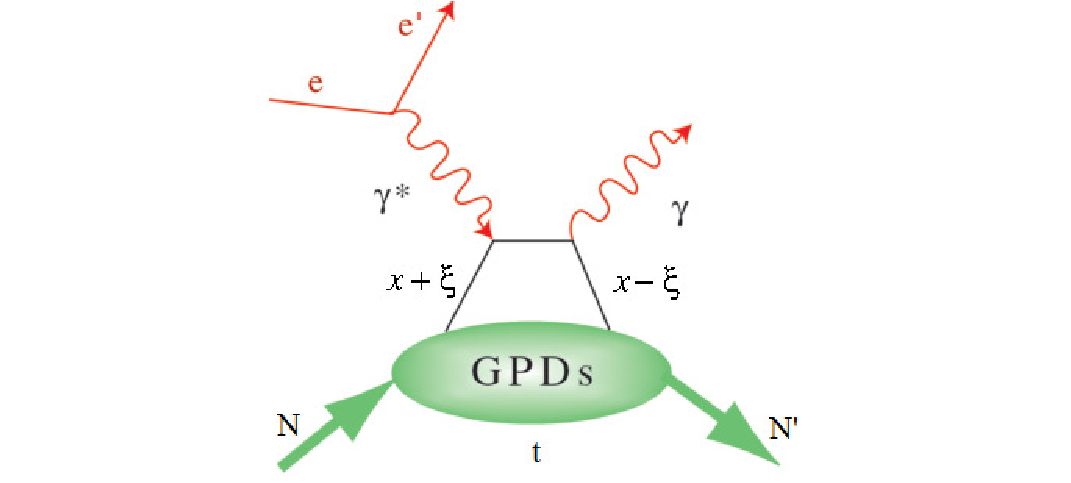
\includegraphics[scale=0.6]{handbag.pdf}
\caption[Handbag diagram for the DVCS process] {The handbag diagram for the DVCS process on the nucleon $eN\to e'N'\gamma'$. 
Here $x+\xi$ and $x-\xi$ are the longitudinal momentum fractions of the 
struck quark before and after scattering, respectively, and $t=(N-N')^2$ is the squared four-momentum transfer between the initial and final nucleons (or equivalently between the two photons).  In the Bjorken limit, i.e. for $Q^2=-q^2=-(k-k^\prime)^2\to \infty$ and $\nu = E_e-E_{e'} \to \infty$ so that the Bjorken scaling variable $x_B$ is finite, $\xi$ is proportional to $x_B$ ($\xi\simeq\frac{x_B}{2-x_B}$, where $x_B=\frac{Q^2}{2M\nu}$, $M$ is the nucleon mass and $\nu$ is the difference between the energies of the initial and final electron in the lab frame).}
\label{fig:dvcs}
\end{center}
\end{figure}

The GPDs depend upon three variables, $x$, $\xi$ and $t$: $x+\xi$ and $x-\xi$ are the longitudinal momentum fractions of the struck quark before and after scattering, respectively, and $t$ is the squared four-momentum transfer between the initial and final nucleon (see caption of Fig.~\ref{fig:dvcs} for the definitions of these variables). The transverse component of $t$ is the Fourier-conjugate variable of the transverse position of the struck parton in the nucleon. Among the three variables, $x$, $\xi$ and $t$, which appear in the DVCS formalism, only $\xi$ and $t$ are experimentally accessible in these reactions. 

The DVCS amplitude is proportional to combinations of integrals over $x$ of the form: 
\begin{equation}\label{dvcs-ampl}
\int_{-1}^{1} d x F(\mp x,\xi,t)\left[\frac{1}{x - \xi + i \epsilon}\pm\frac{1}{x + \xi - i \epsilon}\right]
\end{equation}
where $F$ represents one of the four GPDs. The top combination of the plus and minus signs applies to the quark-helicity independent, or unpolarized, GPDs ($H, E$), and the bottom combination of signs applies to the quark-helicity dependent, or polarized, GPDs ($\widetilde {H}, \widetilde {E}$). Each of these 4 integrals, which are called Compton Form Factors (CFFs), can be decomposed into their real and imaginary parts, as
\begin{eqnarray}\label{def_cffs1}
\Re{\rm e}{\cal F} (\xi,t)&=& {\cal P}\int_{-1}^{1}dx\left[\frac{1}{x-\xi}\mp\frac{1}{x+\xi}\right]F(x,\xi,t) \\
\Im{\rm m}{\cal F}(\xi,t)&=& -\pi [F(\xi,\xi,t)\mp F(-\xi,\xi,t)], \label{def_cffs2}
\end{eqnarray}

where ${\cal P}$ is Cauchy's principal value integral and the sign convention is the same as in Eq.~\ref{dvcs-ampl}. The information that can be extracted from the experimental data at a given ($\xi,t$) point depends on the observable involved. 
$\Re{\rm e}{\cal F}$ is accessed primarily measuring observables which are sensitive to the real part of the DVCS amplitude, such as double-spin asymmetries, beam-charge asymmetries or unpolarized cross sections. 
$\Im{\rm m}{\cal F}$ can be obtained measuring observables which are mainly sensitive to the imaginary part of the DVCS amplitude, such as single-spin asymmetries or cross-section differences. 

However, knowing the CFFs does not define the GPDs uniquely. A model input is necessary to deconvolute their $x$ dependence.

The DVCS process is accompanied by the Bethe-Heitler (BH) process, in which the final-state real photon is radiated by the incoming or scattered electron and not by the nucleon itself. The BH process, which is not sensitive to the GPDs, is experimentally indistinguishable from DVCS and interferes with it at the amplitude level. However, considering that the nucleon form factors are well known at small $t$, the BH process is precisely calculable.
